% $Id: loadproject.tex 6092 2007-11-27 13:25:32Z alexandra $
% Local Variables:
% ispell-check-comments: nil
% Local IspellDict: american
% End:
% --------------------------------------------------------
% User documentation
% copyright by BREDEX GmbH 2005
% --------------------------------------------------------

\index{Project!Open}
\index{Open Project}

\begin{enumerate}
\item To open a \gdproject{} from the database, select:\\
\bxmenu{Test}{Open}{}{}. 
\item If you haven't already logged into the database, a dialog will appear to ask you to do so.  See the previous section \bxpref{tasksdblogin} for details. 
\item Choose the \gdproject{} you want to open from the combo box in the dialog which appears (\bxfigref{loadfromdb}). 

\begin{figure}
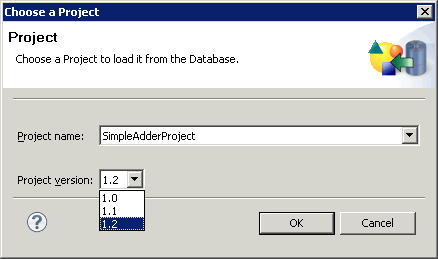
\includegraphics{Tasks/Projects/PS/loadfromdb}
\caption{Open \gdproject{} from \gddb{}}
\label{loadfromdb}
\end{figure}

\item If the \gdproject{} has more than one version, choose which version you want to open. For more information on \gdproject{} versions, see the section later \bxpref{projectversion}. 
\item The \gdproject{} is opened in the \ite{}. 
\end{enumerate}

\subsubsection{Auto loading a default \gdproject{}}
\label{TasksAutoLoadProject}
\begin{enumerate}
\item Use the checkbox in the \bxname{Open Project} Dialog to specify that you want to open this \gdproject{} in this version automatically when you select:\\
\bxmenu{Project}{Open}{}\\
This is useful if you only have one \gdproject{} that you work with.
\item Per workspace, you can have one default \gdproject{}. If you are connected to a \gddb{} which does not contain the \gdproject{}, or if the \gdproject{} is no longer in the \gddb{}, then you will be shown the \bxname{Open Project} Dialog and can choose another \gdproject{}. 
\item In the Test preferences \bxpref{gdprefs}, you can disable the auto load of the \gdproject{}. Doing this will mean that you see the normal  \bxname{Open Project} Dialog when you select\\
 \bxmenu{Project}{Open}{}\\
\end{enumerate}


  
